\documentclass{article}
\usepackage{graphicx}

\begin{document}

\section{General Notes}
There is a model on mother earnings ranges divided into 4 scales ( see Gelman page 67)
once the model has been fit, the following coefficients have been estimated:
\begin{equation}
s = 82.0 + 3.8 \cdot w_2 + 11.5 \cdot w_3 + 5.2 \cdot w_4
\end{equation}
Observe that $w_1$ is missing from the equation, and its predicted score value is the intercept ( and other values being equal to zero).
There is a nice example in Gelman page 53 on how different units affect coefficient interpretation. Compare the following

\begin{equation}
earnings = -61000 + 51 \cdot height[in millimetres] + \epsilon
\end{equation}
And
\begin{equation}
 earnings = -61000 + 81000000 \cdot height[in miles] + \epsilon
\end{equation}

It has been given that standard deviation of height is equal to 3.8 inches, which is 97 millimetres or 0.000061 miles. Observe that we obtain the same expected difference in earnings for the matching units
\begin{equation}
51 \cdot 97 = 81000000 \cdot 0.000061 = 4900
\end{equation}

\section{Scaling}

Suppose there is this model
\begin{equation}
\log_earn = height + male
\end{equation}
Once we fit a linear regression model we have received the following coefficients:
\begin{equation}
\log_earn = 8.153 + 0.021height + 0.423male
\end{equation}
Also,
\begin{equation}
 \exp(0.021) = 1.02
\end{equation}
Therefore, for two people of the same gender one inch of height contributes towards $2\%$ of salary increase. Say that the standard errors are as follows:
\begin{tabular}{|c|c|c|}
\hline 
intercept& height & male \\ \hline 
0.603 & 0.009  & 0.072\\ 
\hline 
\end{tabular} 
\\
\indent
The regression model has a residual standard deviation of $0.88$, implying that approximately $68\%$ of log earnings will be within $0.88$ of the predicted value. As a result, a 70-inch tall person will have earnings equal to $8.153 + 0.021 \cdot 70 = 9.623$. Knowing that predictive standard deviation is $0.88$, there is $68$ chance the person earning are within $9.623 +/- 0.88= [8.74, 10.50]= [\exp(8.74), \exp(10.50)] = [6000, 36000]$. The $R^2$ value for this model was pretty low therefore it is expected to observe such a wide salary range.
\subsection{General approach to standarization}
On another note, we should always standarize the input data to make the interpretation easier.As a result, when analysing the output coefficients, the requirements for other variables being zero is equal to say they are at their averages. There is an example on page 96 that talks about this scenario.
\begin{equation}
s = \beta_0 + \baeta_1 \times d + \baeta_2 \times a + \baeta_3 \times da,
\end{equation}
where $s$ is the probability of switching between wells, $d$ is the distance to the closest well, $a$ is the arsenic level and $da$ is the interaction term between distance and arsenic level.
\\
\indent
The model came out to be
\begin{equation}
s = 0.35 + -0.88 \times d + 0.47 \times a  -0.18 \times da,
\end{equation}
Therefore, the probability of switching when the distance and arsenic level are at their average is equal to $logit^{-1}(0.35) = 0.59$. For distance, we apply the divide by four rule and obtain $-0.88 / 4 = -0.22$. Therefore, at the mean level of arsenic in wells, adding 100 meters to distance will correspond to a negative $0.22$ to probability of switching. Following with arsenic level, we receive that each unit of it, will increase the probability of switching by $0.47 / 4 = 0.12$ when the wells are at the average distance from the household. The interaction term can be interpreted in 2 different ways, always adding a negative $-0.18$ value to the probability of switching. Interaction term can be analysed from two different approaches:
\begin{itemize}
\item distance - for each unit of distance; i.e. 100 meters, a value of $-0.18$ is added to the value of arsenic coefficient. Therefore, because the sign of distance coefficient is negative, we can say that by increasing the arsenic level, \textit{the strength} or \textit{the importance} of the distance prediction \textit{increases} accordingly.
\item arsenic - for each unit of arsenic;  a value of $-0.18$ is added to the value of distance coefficient. Therefore, because the sign of arsenic coefficient is positive, we can say that by increasing the distance to the closes safe well, \textit{the strength} or \textit{the importance} of the distance prediction \textit{decreases} accordingly.
\end{itemize}
\\
\indent

\section{Interaction}

Consider the following model
\begin{equation}
\log( earnings ) ~ (height)
\end{equation}
Once we have fit the equation coefficients given data we obtain the following:
\begin{enumerate}
\item intercept - 5.74
\item height - 0.06
\end{enumerate}
The difference of $0.06$ in height corresponds to $\exp(0.06)=1.062$. Therefore, a unite change of $\beta_1$ corresponds to a $6\%$ increase in the $y$ value. The opposite holds for negative values (i.e there is $6\%$ decrease in the outcome value for a drop of one unit in $\beta_1$). Observe that It would be interesting to see if gender distinction contributes to the $6\%$ increase.

Suppose there is this equation
\begin{equation}
\log(e) = 8.4+0.017 \cdot h - 0.079 \cdot m + 0.007 \cdot h \cdot m 
\end{equation}
where $e$ corresponds to earnings, $h$ height, $m$ to male and $h \cdot m $ it an interaction term between height and male. Now, observe that male intercept does not really have a proper interpretation as it expects the height being equal to 0. However, the interaction term corresponds to the `` difference in the slopes for log earnings between men and women''. Therefore, in interaction term gives us $0.7\%$ increase for men for an inch increase in their height. Moreover, for men and inch increase in hight predicts $1.7\% + 0.7\% = 2.4\%$

\section{Logistic Regression}
Gelman notes on page 81 that ``As with linear regression, the intercept can only be interpreted assuming zero values for the other predictors.'' Observe that this enforces the analyst to look at another point of reference. In other words, if there is equation with only one predictor $x$, we could analyse the predicted value at $\bar{x}$, or any other meaningful point. By meaningful, we are saying values that are observed in the data. In the example provided in the book the equation is given as 
\begin{equation}
logit^{-1} = -1.40 + 0.33x
\end{equation}
What we can do is pick two consecutive units of $x$ and then report the percentage change, given the unit difference
\\
\indent
It is assumed on page 83 that coefficient estimates within two standard errors from the estimated coefficient value are consistent with data. However, a statistically significant coefficient is required to be at least 2 standard errors \textbf{away from zero}.
\\
\indent
This is also reported on pages 90-91 when there is a following model presented:

\begin{equation}
 s = -0.9 \cdot d + 0.46 \cdot a,
\end{equation}

where $s$ is probability of switching between two wells, $d$ is the distance to the nearest well in meters ( divided by 100), $a$ is the arsenic level of the currently used well. Intercept has been estimated as very close to $0$. With the quick application of the dive by 4 rule, we could see that for the same arsenic level, $100m$ corresponds to $-0.22$ probability of switching. Similarly, one unit difference on the arsenic scale corresponds to $11\%$ to probability of switching. What this means is that the closer the safe well is - the easier it is for household to switch. In addition, the higher the arsenic level, the more probable it is to switch.
\\
\indent It is very important to note that we cannot claim that distance is more of an influential factor than arsenic level.What we should do instead is to investigate how one standard deviation change in data affects the probability of switching. As a result, we will be able to report on differences in ``common units''. Standard deviations are equal to $ \sigma_d = 0.38$, $\sigma_a = 1.1$, which yields  $-0.9 \cdot 0.38 = -0.34$, and $0.46*1.10=0.51$. Now, we can apply the divide by 4 rule on the estimated data. Thus, a $\sigma_d$ change in distance corresponds to $-8\%$ (negative) difference to the probability of switching, while a $\sigma_a$ change in arsenic level gives $13\%$ in the probability of switching.

\subsubsection{UCLA datasets}
There is a good introduction to logistic regression on UCLA website. There is a dataset that contains test results split between two genders. This is the gender distribution:
\begin{enumerate}
\item female - 109
\item male - 91
\end{enumerate}
The first analysis is to run a logistic regression to check how many students finish their class with honorous distinction.
\\
\begin{tabular}{|c|c|c|}
\hline 
& H & N \\ 
\hline 
F & 32 & 77 \\ 
\hline 
M & 17 & 74 \\
\hline 
\end{tabular} 
\\
We would like to run a logistic model to regress gender onto class type:
\begin{equation}
 h = \beta_0 + \beta_1g
\end{equation}
where $h$ represents the class that students attended and $g$ is gender.
The equation is estimated as
\begin{equation}
 h = -1.4709 + 0.5928g
\end{equation}
Observe that $\exp(-1.4709) = 0.2297$. The odds of being in honorous class for males is $\frac{17}{74}=0.2297 $, which is the same as the exponent of the intercept. Therefore, the estimated intercept is equal to ratio of the reference group (i.e. male) belonging to the honorous class.
\\
\indent Recall, that the ratio of female students attending a honorous class is $\frac{32}{77}$. As a result, the ratio of the odds of females to males is 
\begin{equation}
 \frac{\frac{32}{77}}{\frac{17}{74}} = 1.8090
\end{equation}, which is the same as the exponent of the coefficient of female $\exp(0.5928) = 1.8090$.
\\
\indent
Subsequently, we could analyse a model in which math scored is regress on whether the students have attended a honorous class or not, as in:

\begin{equation}
 h = \beta_0 + \beta_1m  ,
\end{equation}
where $m$ is math score, and $h$ a math score.

%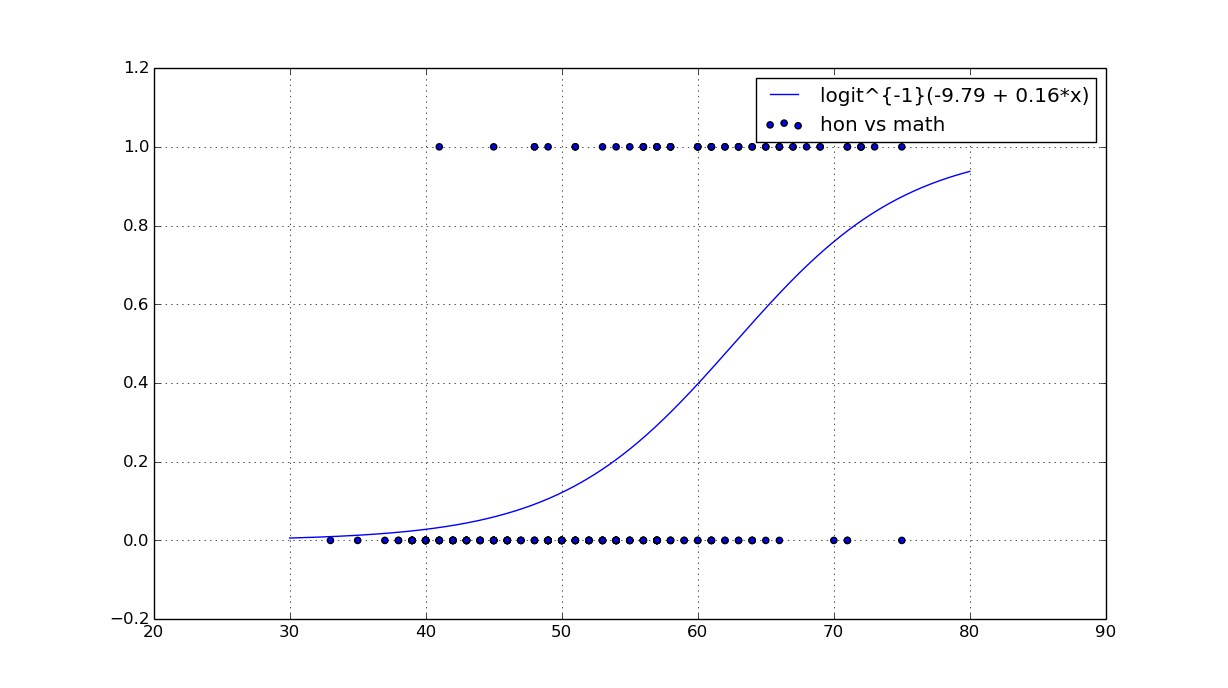
\includegraphics[scale=0.2]{hon_math_logit.png}

Obviously this works well for two binary options. Suppose there is $k-$level categorical variable denoting earnings and it regress on a candidate selection during national elections. Therefore, Gelman on pages 82-82 talks about mathematical approach given the estimated formula. These are the potential solutions
\begin{itemize}
\item "Divide by four" - it turns out that if we calculate $\beta \ 4 $ we will get a pretty good estimate of what the percentage of change is given a unit change for a variable.
\item Unit change - in this approach we plug in 2 consecutive units into the regression equation, and look at the percentage change.
\item latent approach - defined as an observable set of pairs
\begin{equation}
(y_i, X_i\beta + \epsilon)
\end{equation}
where $y \in \{0,1\}$, and $y_i = 1,$ when $X_i\beta + \epsilon >0$ and $y_i = 0$ otherwise. Error terms are assumed to have logistic distribution. Also, error term follows Gaussian distribution with $\mu = 0$ and $\sigma = 1.6$
\begin{equation}
 \epsilon  N(0, \sigma^2)
\end{equation}
\end{itemize}
%\begin{array}{ccc}
% & H & N \\ 
%F & 32 & 77 \\ 
%M & 17 & 74 \\
%\end{array}

\end{document}